\section{Area Between Curves}
\begin{itemize}
    \item Suppose we wish to find the area between two curves $f(x)$ and $g(x)$. We can do this by partitioning the area into infinitesimally small rectangles:
    \begin{equation}
        \Delta A_i = [f(x_i^*)-g(x_i^*)]\Delta x_i
        \label{eq:}
    \end{equation}
    so that the area is given by:
    \begin{align}
        A &= \lim_{\lVert P \rVert \to 0} \sum_{i=1}^n \left[f(x_i^*)-g(x_i^*)\right]\Delta x_i \\ 
        &= \int_a^b\left[f(x)-g(x)\right]\dd{x}
    \end{align}
    If we let 
    $f(x)\ge g(x)$ when $x\in[a,b]$, then this gives the difference in their areas $A_1-A_2$.
    \item If the condition $f(x)\ge g(x)$ is not satisfied, then we must break up the integral into multiple parts (if we interpret the area as having a positive area only). We can modify the area formula to be:
    \begin{equation}
        A = \int_a^b |f(x)-g(x)| \dd{x}
        \label{eq:}
    \end{equation}
    \item Suppose we have a curve $x=f(y)$ and $x=g(y)$ instead. The area between $y=a$ and $y=b$ works in the same way:
    \begin{equation}
        A = \int_a^b |f(y)-g(y)| \dd{y}
        \label{eq:}
    \end{equation}
    \item If we instead have two inequalities, we are flexible to choose any method. 
    \begin{example}
        What is the area contained within:
        \begin{align}
            x-2y^2\ge 0 \\ 
            1-x-|y| \ge 0
        \end{align}
        We can plot these two inequalities (sorry I don't know how to shade in regions in \LaTeX):
        \begin{center}
        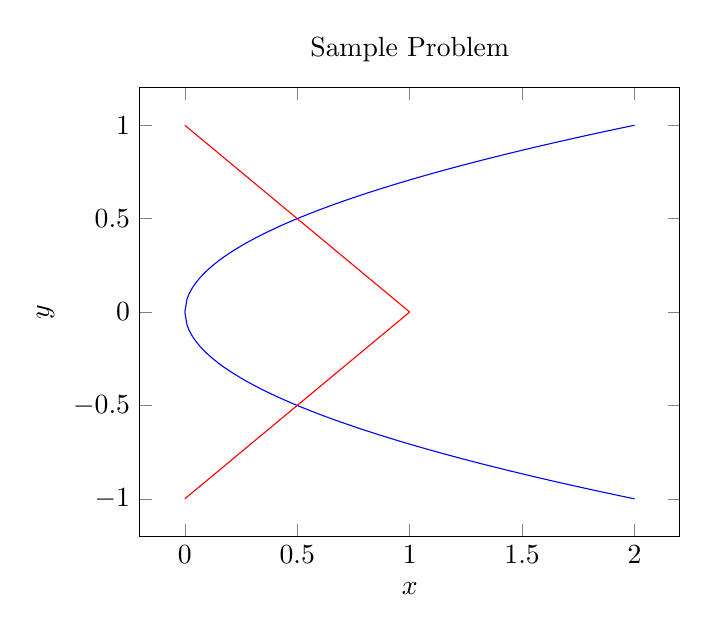
\begin{tikzpicture}
        \begin{axis}[
        legend pos=outer north east,
        title=Sample Problem,
        axis lines = box,
        xlabel = $x$,
        ylabel = $y$,
        variable = t,
        trig format plots = rad,
        ]
        \addplot [
            domain=0:2,
            samples=200,
            color=blue,
            ]
            {(x/2)^0.5};
        \addplot [
            domain=0:2,
            samples=200,
            color=blue,
            ]
            {-(x/2)^0.5};
        \addplot [
            domain=0:1,
            samples=200,
            color=red,
            ]
            {1-x};
        \addplot [
            domain=0:1,
            samples=200,
            color=red,
            ]
            {x-1};
        \end{axis}
        \end{tikzpicture}
        \end{center}
        We can integrate with respect to $y$ by noting that it is symmetric around the $x$ axis. Then the two curves become:
        \begin{align}
            x &= 1-y \\ 
            x &= 2y^2
            \label{eq:}
        \end{align}
        for $-\frac{1}{2} \le y \le 0$. Then the area is:
        \begin{align}
            A &= 2\int_0^{1/2} \left(1-y-2y^2\right)\dd{y} \\ 
            &= 2\left(y-\frac{y^2}{2}-\frac{2y^3}{3}\right)\Big|^{1/2}_0 \\ 
            &= 2\left(\frac{1}{2}-\frac{1}{8}-\frac{1}{12}\right) \\ 
            &= \frac{7}{12}
        \end{align}
    \end{example}
\end{itemize}